\documentclass{article}

\title{Baseball Research Log}
\author{Chris Comiskey}
\date{Winter 2017}

\usepackage{natbib}
\bibliographystyle{unsrtnat}

\usepackage{fullpage}
\usepackage{ulem}

\usepackage{amsmath, amsthm, amssymb, amsfonts}
\usepackage{mathtools}
\usepackage{float}
\usepackage{bbm}

\usepackage{listings}


\begin{document}

\maketitle{}

\section*{Week of December 5, 2016} % ========================
\begin{itemize}
\item An option:
      \begin{itemize}
      \item Started with $\pmb{\beta} \sim \text{N}(\pmb{0}, 5 \text{{\bf I}}_{6})$ non-informative prior 
      \item ...Define $\pmb{\theta} = \pmb{R \beta}$
      \item ...giving Var$(\pmb{\theta}) = \pmb{R}\text{Var}(\pmb{\beta})\pmb{R}'$
      \item Then use prior distribution $\pmb{\theta} \sim \text{N}(\pmb{R \hat{\beta}}, 5 *\pmb{R R'})$ (...but diagonal only)
      \end{itemize}
\item \verb|Hitter6.stan|. Used $\pmb{R}$ and polar $\hat{\pmb{\beta}}_{\text{GLM}}$ to estimate $\text{E}[\pmb{\theta}]$ and $\text{Var}[\pmb{\theta}]$, as in previous bullet point.
\begin{verbatim}
data {                             
  int<lower=0> N;                 // Number of observations
  int<lower=0> p;                 // number of predictors
.
.
.
      Z ~ normal(0, 1);  // Each element is N(0,1)
      Z_mod = Sigma * Z; // (Cov matrix Cholesky)*MVN(0,1)
      hit ~ bernoulli_logit(beta0 + Q*theta + Z_mod);
}
\end{verbatim}
\item Reading \cite{Finley2007}
\item Also looking at Andy's notes from NCAR. 
\item Reading slides titled ``functional-casestudy.pdf''
\item Idea: could define $\beta$ in \verb|Hitter6.stan| as $\hat{\beta}_{\text{GLM}}$, to get idea of length-scale ballpark.
\item Alarming question: is Z a parameter?
\item Ran \verb|Hitter5.stan| overnight, for N = 2000. Only made it through 350 samples. Prohibitive.
\item Gotta try sampling loop. For i in 1:100, sample 200, fit with \verb|Hitter5.stan|, then compile all those draws. Would that work/help?
\item Reading \cite{Neal2011} to learn about Hamiltonian MCMC (HMC) algorithm, which Stan uses. Hamiltonian Dynamics; Mr. Meyers would be proud.
\item Wikipedia:  ``In mathematics, the {\bf gradient} is a generalization of the usual concept of derivative to functions of several variables.'' 
\item What if I used my variable resolution grid to estimate variance parameters? 
  \begin{itemize}
  \item Using the usual box centers reduction would be shoddy because many boxes would have very little data, and thus misrepresent Cov(Box1, Box2). 
  \item For example, $\hat{p}_{\text{Box1}} = 1$ for one out of one, against $\hat{p}_{\text{Box2}} = 0.12$ for 12 out of 100, misrepresents Cov(Box1, Box2). 
  \item Using my variable resolution grid would offer advantages, by eliminating $\hat{p}_{\text{Box1}} = 1$ scenarios.
  \end{itemize}
\end{itemize}

\subsection*{Meeting}
\begin{itemize}
\item Alix was worried, because I wanted to meet {\it this week}, that I had found a job and was going to leave early! She said she has had other students do the same, and it is very hard to finish in that fashion.
\item Alix read my paper, made some comments, said it was good. She thinks at the end there should be a section of sorts that helps the (baseball) reader understand and interpret the new map, rather than than just understanding the algorithm. What do the box sizes tell us? What does the particular spatial variation in box size tell us? 
\item Alix is thinking space might be a dual stopping criteria. For example, can hitters even distinguish pitches in two adjacent very small boxes? They probably look like the identical pitch, so why assign separate batting averages.
\item ``Banish from your mind'' the question of whether or not this is PhD level research. She said there is {\bf no way anyone below the PhD level could make their way through} (i) Finley's papers, (ii) the  QR decomposition of $\pmb{X \beta}$ (linear model theory) in my logistic regression model (GLM) and the resultant change in the prior distributions (Bayesian-LMT), or (iii) MCMC with Hamiltonian dynamics, etc (just the stuff we talked about today). And, she said, it's very cool we're applying it to something totally different (other than forestry, etc), baseball, where it totally applies. Bottom line: {\bf Alix is sure.} She's my primary adviser. ``God,'' as Bruce put it. Her opinion carries all the weight. The jury starts and stops with her. She believes it, I get a PhD.
\item Can always contact Andy and/or Malcom is needbe
\item Need to try leaving $\theta \sim N(\pmb{0}, 5*\pmb{R*R^{T}})$. In other words, shoul be fine to leave the mean uninformative if adjust variance.
\item Okay that $\theta$s correlated according to $Var(\theta) = 5*\pmb{R*R^{T}}$ because coefficient estimates always are, even in simple linear regression.
\item My idea of using variable resolution grid to change grid-reduced estimates of correlation parameters is worth coming back to. She wasn't sure if the base method existed (or not) to improvise upon.
\end{itemize}

\subsection*{Carrying on...}
\begin{itemize}
\item As mentioned above. Correct adjusted prior variances on $\hat{\theta}$, with mean zero. \verb|Hitter5WOSC|
\begin{verbatim}
> print(fit_hitterWOSC, pars=c("beta0","beta"), digits = 3)
Inference for Stan model: Hitter5WOSC.
3 chains, each with iter=500; warmup=250; thin=1; 
post-warmup draws per chain=250, total post-warmup draws=750.

          mean se_mean    sd   2.5%    25%    50%    75%  97.5% n_eff  Rhat
beta0   -4.068   0.055 0.682 -5.475 -4.516 -4.066 -3.627 -2.800   155 1.015
beta[1]  1.168   0.038 0.487  0.219  0.847  1.150  1.473  2.228   168 1.014
beta[2] -1.929   0.127 1.874 -5.803 -3.199 -1.812 -0.535  1.314   217 1.008
beta[3] -0.316   0.006 0.086 -0.494 -0.369 -0.315 -0.261 -0.149   236 1.009
beta[4] -3.978   0.064 1.093 -6.225 -4.742 -3.910 -3.187 -2.059   290 1.006
beta[5] -1.691   0.059 0.887 -3.357 -2.289 -1.722 -1.065  0.106   229 1.008
beta[6] -0.471   0.013 0.212 -0.861 -0.618 -0.483 -0.321 -0.056   282 1.006
\end{verbatim}
As they should be! They match the plane Jane GLM fit without spatial correlation random effect. 
\item \verb|Hitter5WOSC.stan|
\begin{verbatim}
data {                             
  int<lower=0> N;                 // Number of observations
  int<lower=0> p;                 // number of predictors
  matrix[N,p] Q;                  // QR decomp - Q
  matrix[p,p] R;                  // QR decomp - R
  int<lower=0, upper=1> hit[N];   // 0/1 outcomes; array of integers
  vector[p] theta_SDs;            // theta prior SDs
}
transformed data{
  matrix[p,p] R_inv;
  R_inv = inverse(R);
}
parameters {                
  real beta0;                       // intercept 
  vector[p] theta;
}
transformed parameters {
      vector[p] beta;
      beta = R_inv*theta;
}
model {  
      beta0 ~ normal(0,5);
      theta[1] ~ normal(0, theta_SDs[1]);
      theta[2] ~ normal(0, theta_SDs[2]);
      theta[3] ~ normal(0, theta_SDs[3]);
      theta[4] ~ normal(0, theta_SDs[4]);
      theta[5] ~ normal(0, theta_SDs[5]);
      theta[6] ~ normal(0, theta_SDs[6]);
      hit ~ bernoulli_logit(beta0 + Q*theta);
}
\end{verbatim}

\item {\bf Ask Alix:} Try sampling loop... For i in 1:100, sample 200, fit with \verb|Hitter5.stan|, then compile all those draws. Would that work/help?
\end{itemize}

\section*{Week of January 9, 2017} % ========================
\begin{itemize}
\item Where was I?
  \begin{enumerate}
  \item STAN needs to go faster; enter Andrew Finley
  \item Andrew Finley, reduce dimensionality of correlation
  \item Paper; Alix edits/feedback to look at
  \item Expand picture effort to include 3D representation of CIs
  \item Hamilton equations
  \end{enumerate}
\item Confirmed: Using 9177 obs, QR decomposition, and QR inflated variances, but leaving out spatial correlation, all incorporated into \verb|Hitter5WOSC.stan| yields same estimates as \verb|glm()|. So stan code is working, and QR decomposition is working. As of now, running the same procedure WITH spatial correlation is prohibitively slow.

\end{itemize}

\subsection*{MCMC Using Hamiltonian Dynamics \citep{Neal2011}}
\begin{itemize}
\item Paraphrased: MCMC originated with (Metropolis et al. 1953) to simulate states for molecules... another approach (Alder and Wainwright, 1959) formalized Newton’s laws of motion as Hamiltonian dynamics.
\item Duane et al. 1987 paper united approaches as Hybrid MC, or Hamiltonian MC $\rightarrow$ HMC for lattice field theory quantum dynamic simulations. 
\item Statistical use began in 1996 with neural network models, other applications followed.
\item Differential equations and ``leapfrog'' scheme, elementary mathematics

\end{itemize}
Steps.
      \begin{enumerate}
      \item ``Define a Hamiltonian function in terms of the probability distribution we wish to sample from.''
      \item Interested in ``position'' variables. Introduce auxiliary ``momentum'' variables (typically independent Gaussian distributions)
      \item The HMC method alternates:
        \begin{enumerate}
        \item Simple updates for these momentum variables 
        \item Metropolis updates - computing Hamiltonian dynamic trajectory for new proposal state, leapfrog implementation method, distant proposals w/ high acceptance probability; bypass slow random walk proposal distribution
        \end{enumerate}
      \end{enumerate}
\begin{itemize}
\item Physical interpretation - frictionless puck on varying height surface. Puck at {\bf position} $q$ with {\bf momentum} $p$ and mass $m$, {\bf potential energy} $U(q)$, {\bf kinetic energy} $K(p) = |p|^{2}/(2m)$.
\item Wikipedia: ``In statistics, especially in Bayesian statistics, the {\bf kernel} of a probability density function (pdf) or probability mass function (pmf) is the form of the pdf or pmf in which any factors that are not functions of any of the variables in the domain are omitted.''
\end{itemize}

\subsubsection{Equations}
\begin{itemize}
\item q = position, U(q) = potential energy 
      \begin{itemize}
      \item \pmb{q} = variables of interest
      \item let $U(q) = -\text{log}f_{q}(q)$
      \end{itemize}
\item p = momentum, K(p) = kinetic energy
      \begin{itemize}
      \item Introduce artificially, same dimension as \pmb{q}
      \end{itemize}
\item Partial derivatives determine change over time. For $i = 1,\dots, d$:
$$ \frac{d q_{i}}{dt} = \frac{\partial H}{\partial p_{i}}$$
$$ \frac{d p_{i}}{dt} = -\frac{\partial H}{\partial q_{i}}$$

\item $H(q,p) = U(q) + K(p) = -\text{log}f_{q}(q) + p^{T}\pmb{M}^{-1}p/2$
    \begin{itemize}
    \item Total = Potential + Kinetic
    \item $U(q) = -\text{log}f_{q}(q)$
    \item $K(p) = -\text{log }f_{p}(p) = p^{T}\pmb{M}^{-1}p/2$, (using p $\sim$ N(0,\pmb{M}))
    \end{itemize}
\item Rewrite:
$$ \frac{d q_{i}}{dt} = \frac{\partial H}{\partial p_{i}} = [\pmb{M}^{-1}p]_{i}$$
$$ \frac{d p_{i}}{dt} = -\frac{\partial H}{\partial q_{i}} =- \frac {\partial U}{\partial q_{i}} $$
\item Solution: q(t) = ?, p(t) = ?
\end{itemize}

\section*{Week of January 17, 2017} % ========================

\subsection*{Hamiltonian Mechanics/Dynamics }
\begin{itemize}
\item Leapfrog method = for calculating new position (q) and momentum (p) through tiny time steps
  \begin{itemize}
  \item for {\bf discretizing Hamilton equations}
  \item akin to Taylor Series appoximations
  \item Postion (q) (or momentum (p)) at $t_{0}$ plus time step times rate of change of position (q) (momentum (p)) variable at $t_{0}$
  \item Leapfrom Method does half step for momentum (p), full step for postion (q), other half step for momentum (p). Damn good.

  \end{itemize}
\item {\bf Statistical ensemble} - probability distribution for the state of a system (set of all possible copies)
\item Short version: randomly sample from K(p) (kinetic, momentum), calculate U(k) (potential, position*) --- that's your Metropolis proposal.
\item {\bf Solve} a differential equation: If $\frac{dq}{dt} = p$, and $\frac{dp}{dt} = q$, then q(t) = ?, and p(t) = ?
\end{itemize}

\subsection*{Pictures}
Consider this presentation of CIs in 3D. \\
\includegraphics[scale=.4]{Images/FightEntropy.jpg} \\
Note the line segments through the surface. \\
Brainstorming.
\begin{itemize}
\item Could do a {\bf {\it shiny} app (!!)} that gives a $1-\alpha$ slider to move \sout{three-dimensionally} through the CI, showing the lower ($\alpha/2$) and upper bound ($1-\alpha/2$) maps on the left (lower) and right (upper) of the point estimate map. The left and right would converge to middle map (point estimate) for 0\% CI. 
\item Could even... {\bf have option for cutoff(!!)} as part of app! ...and px, pz, CI percentile
\item Could have a profile plot attached, with px or pz on x-axis, $\hat{p}$ on y-axis---with colors. \\
    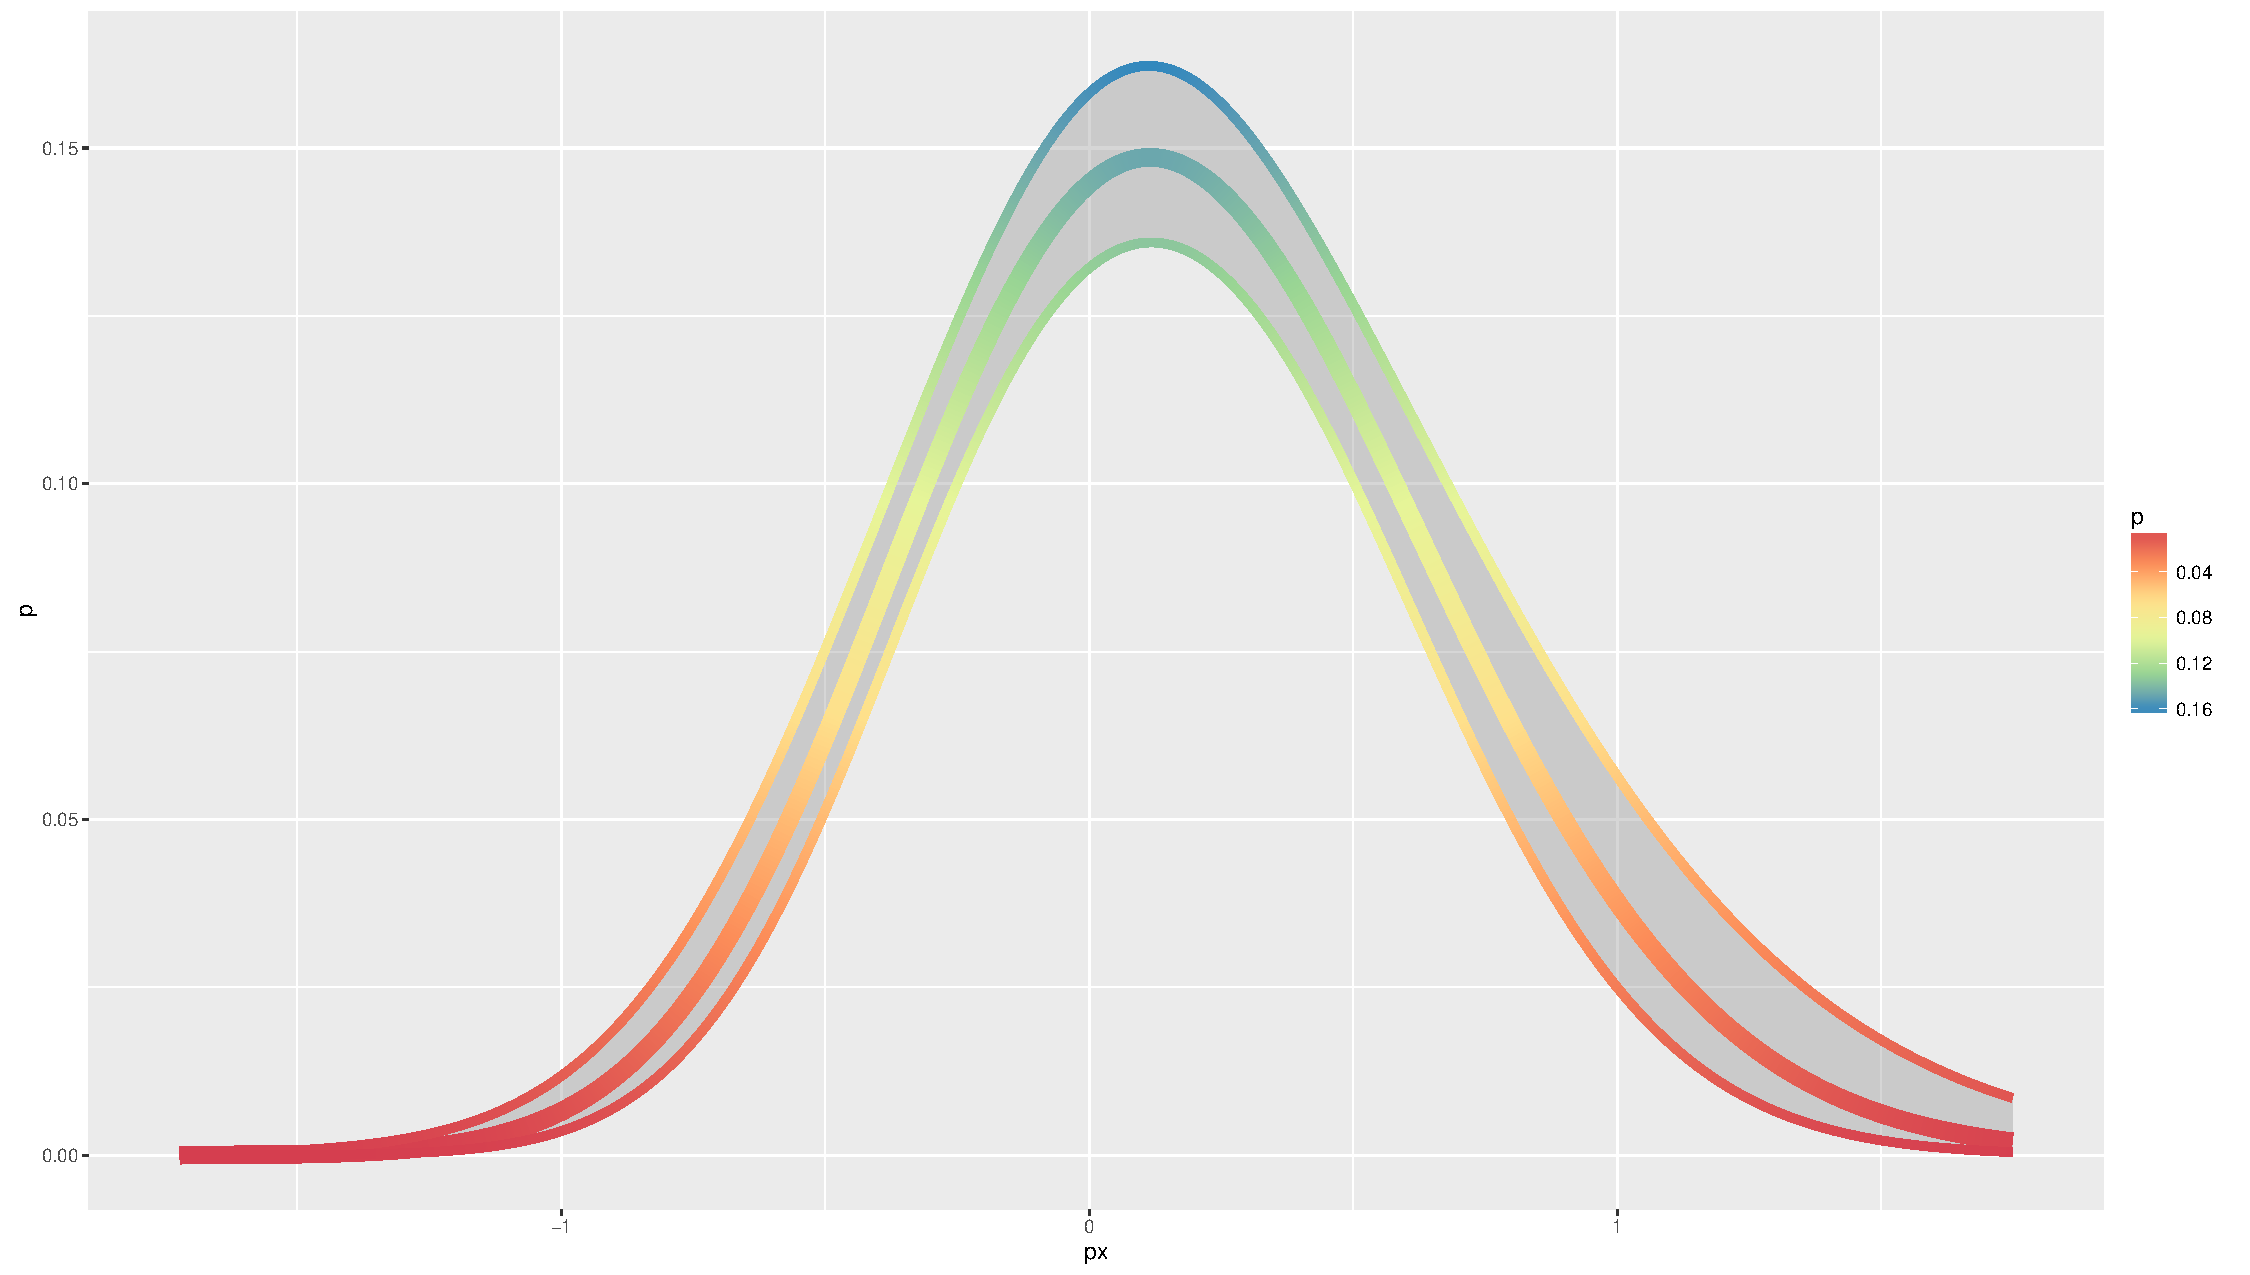
\includegraphics[scale=.2]{Images/PolarGLM_ProfileCI.pdf} 
\item Confusion: In my heat maps, color = $\hat{p}$. In my mental images of  CIs $\hat{p}$ the 3D qualities of height and width represent $\hat{p}$ too. 
\item {\bf shiny} app is the key.
\end{itemize}

\subsection*{Shiny}
  \begin{itemize}
  \item See \verb|Shiny.R|
  \item Tutorials: https://shiny.rstudio.com/tutorial/ 
  \end{itemize}
\subsection*{Lesson 1 - Recap}
To create your own Shiny app:
  \begin{enumerate}
  \item Make a directory named for your app.
  \item Save your app’s \verb|server.R| and \verb|ui.R| script inside that directory.
  \item Launch the app with runApp (button) or RStudio’s keyboard shortcuts (Command+Shift+Enter).
  \item Exit the Shiny app by clicking escape.
  \end{enumerate}
  
\subsection*{Lesson 2 - Build a User Interface}
\begin{itemize}
\item create a user-interface with \verb|fluidPage()|, \verb|titlePanel()| and \verb|sidebarLayout()|
          \begin{verbatim}
      # ui.R
      
      shinyUI(fluidPage(
      
        titlePanel("title panel"),
      
        sidebarLayout(
          sidebarPanel("sidebar panel"),
          mainPanel("main panel")
        )
        
      ))
            \end{verbatim}
\item create an HTML element with one of Shiny’s tag functions; i.e. \verb|h2()|, \verb|br()|, etc.
\item set HTML tag attributes in the arguments of each tag function; i.e. \verb|h2("header", align = "center")|
\item add an element (i.e. \verb|img(...)| or \verb|h2(...)|) to your web page by passing it to  \verb|titlePanel|,  \verb|sidebarPanel| or  \verb|mainPanel|.
\item add multiple elements to each panel by separating them with a comma
\item add images by placing your image in a folder labeled  \verb|www| within your Shiny app directory and then calling the  \verb|img| function (\verb|img(src = "bigorb.png", height = 72, width = 72)|)
\end{itemize}

\subsection*{Lesson 3 - Add Control Widgets}
\begin{itemize}
\item Widget - A web element users can interact with.
\item Widgets have help pages; \verb|?actionButton|
\end{itemize}


\subsection*{Meeting}
\begin{itemize}
\item Dissertation
        \begin{itemize}
        \item Chapter 1: I made the Alix feedback changes (Alix happy), I will add Shiny CI presentation stuff to round it out. Doesn't need to be more technical.
        \item Chapter 2 (and this term): \verb|spbayes()|, fit model with random effect.
        \item Chapter 3: Does random effect improve* model? *How do we measure *improve.
        \end{itemize}
\item Need to brush up on ``credible interval,'' the Bayesian paradigm's answer to confidence intervals.
\item I explained my plan for Shiny app approach to CI. They liked the idea. Alix especially.
        \begin{itemize}
        \item Gameplan is to show CI for variable resolution heat map
        \item And for continuous model {\bf without} random effect, but to only briefly introduce the model at this point, and allude to thorough introduction to come in Chapter 2.
        \end{itemize}
\item Charlotte went to RStudio conference. 
        \begin{itemize}
        \item Mango had a table there, promoting their training mostly (she thinks). 
        \item She said they have fully bought into the Hadley Wickham universe of packages. 
        \item Mango now teaches R by starting with \verb|dplyr|, data frames, etc. 
        \item (This is great news for me!) 
        \item She said Mango was one of the companies on her radar if academia didn't work out!
        \end{itemize}
\item Alix asked: ``Is HMC what \verb|spbayes()| uses?'' 
        \begin{itemize}
        \item I don't know, but I don't need to own Hamiltonian dynamics if \verb|spbayes()| doesn't use it. Good point Alix. 
        \end{itemize}
\end{itemize}


\section*{Week of January 23, 2017} % ========================

\subsection*{Lesson 4 - Reactive *Output*}
\begin{itemize}
\item Use an \verb|*Output| (e.g. \verb|textOutput(...)|) function in the \verb|ui.R| script to place reactive objects in your Shiny app
\begin{verbatim}
# ui.R

shinyUI(fluidPage(
  titlePanel("censusVis"),
  
  sidebarLayout(
    sidebarPanel(
      helpText("Create demographic maps with 
               information from the 2010 US Census."),
      
      selectInput("var", 
                  label = "Choose a variable to display",
                  choices = c("Percent White", "Percent Black",
                              "Percent Hispanic", "Percent Asian"),
                  selected = "Percent White"),
      
      sliderInput("range", 
                  label = "Range of interest:",
                  min = 0, max = 100, value = c(0, 100))
      ),
    
    mainPanel(
      textOutput("text1"),  # **Notice "output$text1"
      textOutput("text2")
    )
  )
))
\end{verbatim}
\item Use a \verb|render*| function in the \verb|server.R| script to tell Shiny how to build your objects
\begin{verbatim}
# server.R

shinyServer(function(input, output) {

  output$text1 <- renderText({            # **Notice "output$text1"
    paste("You have selected", input$var) # **Notice "input$var"
    }) 
    
  # ** Notice "output$text2" contains "input$range[1]"  
  output$text2 <- renderText({
    paste("Your range is", input$range[1], "to", input$range[2])
  })
    
})
\end{verbatim}
\item Surround R expressions by braces, {}, in each \verb|render*| function
\item Save your \verb|render*| expressions in the output list, with one entry for each reactive object in your app.
\item Create reactivity by including an input value in a \verb|render*| expression
\end{itemize}

* Workflow seems to me: \verb|ui.R| takes {\bf input} $\longrightarrow$ \verb|server.R| receives {\bf input} and creates {\bf output} $\longrightarrow$ \verb|ui.R| displays {\bf output}.

* Reactivity: connect \verb|input| {\it values} to \verb|output| {\bf objects}.

\subsection*{Lesson 5 - Use R Scripts and Data}
\begin{verbatim}
# server.R

  # A place to put code ***

shinyServer(
  function(input, output){
    
      # Another place to put code ***
    
      output$map <- renderPlot({
    
          # A third place to put code ***
          
      )}
      
    }
  )
\end{verbatim}
\begin{itemize}
\item The \verb|server.R| script is run once, when you launch your app
\item The unnamed function inside \verb|shinyServer| is run once each time a user visits your app
\item The R expressions inside \verb|render*| functions are run many times. Shiny runs them once each time a user changes a widget.
\end{itemize}
How can you use this information?
\begin{itemize}
\item Source scripts, load libraries, and read data sets at the beginning of \verb|server.R| outside of the \verb|shinyServer| function. Shiny will only run this code once, which is all you need to set your server up to run the R expressions contained in \verb|shinyServer|.

\item Define user specific objects inside \verb|shinyServer|’s unnamed function, but outside of any \verb|render*| calls. These would be objects that you think each user will need their own personal copy of. For example, an object that records the user’s session information. This code will be run once per user.

\item Only place code that Shiny must rerun to build an object inside of a \verb|render*| function. Shiny will rerun all of the code in a \verb|render*| chunk each time a user changes a widget mentioned in the chunk. This can be quite often.

\item You should generally avoid placing code inside a render function that does not need to be there. The code will slow down the entire app.
\end{itemize}
Recap
\begin{itemize}
\item You can create more complicated Shiny apps by loading R Scripts, packages, and data sets.
\item The directory that \verb|server.R| appears in will become the working directory of the Shiny app
\item Shiny will run code placed at the start of \verb|server.R|, before \verb|shinyServer|, only once during the life of the app.
\item Shiny will run code placed inside \verb|shinyServer| multiple times, which can slow the app down.
\item You also learned that \verb|switch| is a useful companion to multiple choice Shiny widgets. Use switch to change the values of a widget into R expressions.
\end{itemize}

\subsection*{Lesson 6 - Reactive *Expressions*}
Reactive expressions save their calculated value, and only recalculate when a widget input changes.
\begin{verbatim}
# server.R

library(quantmod)
source("helpers.R")

shinyServer(function(input, output) {

  # Use reactive({.}) expression to create object
  dataInput <- reactive({
    getSymbols(input$symb, src = "yahoo", 
      from = input$dates[1],
      to = input$dates[2],
      auto.assign = FALSE)
  })
  
  # Use reactive object in render*({.}) statment
  output$plot <- renderPlot({    
    chartSeries(dataInput(), theme = chartTheme("white"), 
      type = "line", log.scale = input$log, TA = NULL)
  })
})
\end{verbatim}
``When you click the “Plot y axis on the log scale” widget button, \verb|input$log| will change and \verb|renderPlot| will re-execute. Now
      \begin{enumerate}
      \item \verb|renderPlot| will call \verb|dataInput()|
      \item \verb|dataInput| will check that the "dates" and "symb" widgets have not changed
      \item \verb|dataInput| will return its saved data set of stock prices {\it without re-fetching data from Yahoo}
      \item \verb|renderPlot| will re-draw the chart with the correct axis.
      \end{enumerate}
Shiny will automatically re-build an object if
\begin{itemize}
\item an input value in the objects's \verb|render*| function changes, or
\item a reactive expression in the objects's \verb|render*| function becomes obsolete
\end{itemize}
{\bf Reactive expressions save their results, and will only re-calculate if their input has changed.}
\subsubsection*{Lesson 7}
Share your apps...
\begin{itemize}
\item {\bf Shinyapps.io}

The easiest way to turn your Shiny app into a web page is to use shinyapps.io (http://my.shinyapps.io/), RStudio's hosting service for Shiny apps. 

shinyapps.io lets you upload your app straight from your R session to a server hosted by RStudio. You have complete control over your app including server administration tools. You can find out more about shinyapps.io by visiting shinyapps.io (http://my.shinyapps.io/).
\end{itemize}

\subsection*{Finley, Quest for Gaussian Predictive Process Models}
\begin{itemize}
\item This \citep{Finley2009} looks possibly helpful.
\item Bingo. \citep{Finley2009_2}. 
      \begin{itemize}
      \item Abstract: ``...spatially-varying multinomial logistic regression models to predict forest type groups... spatially-varying impact of predictor variables... onerous computational burdens and we discuss dimension reducing spatial processes...''
      \end{itemize}
\item Maybe \citep{Finley2011}
\item Looks cool. \citep{Guhaniyogi2011}
  \begin{itemize}
  \item Large point referenced datasets occur frequently in the environmental and natural sciences. Use of Bayesian hierarchical spatial models for analyzing these datasets is undermined by onerous computational burdens associated with parameter estimation. Low-rank spatial process models attempt to resolve this problem by projecting spatial effects to a lower-dimensional subspace. This subspace is determined by a judicious choice of ‘knots’ or locations that are fixed a priori. One such representation yields a class of predictive process models (e.g., Banerjee et al., 2008) for spatial and spatial-temporal data. Our contribution here expands upon predictive process models with fixed knots to models that accommodate stochastic modeling of the knots. We view the knots as emerging from a point pattern and investigate how such adaptive specifications can yield more flexible hierarchical frameworks that lead to automated knot selection and substantial computational benefits.
  \end{itemize}
\item \citep{Finley2012}
\item \citep{Eidsvik2012}
  \begin{itemize}
  \item The challenges of estimating hierarchical spatial models to large datasets are addressed. With the increasing availability of geocoded scientific data, hierarchical models involving spatial processes have become a popular method for carrying out spatial inference. Such models are customarily estimated using Markov chain Monte Carlo algorithms that, while immensely flexible, can become prohibitively expensive. In particular, fitting hierarchical spatial models often involves expensive decompositions of dense matrices whose computational complexity increases in cubic order with the number of spatial locations. Such matrix computations are required in each iteration of the Markov chain Monte Carlo algorithm, rendering them infeasible for large spatial datasets. The computational challenges in analyzing large spatial datasets are considered by merging two recent developments. First, the predictive process model is used as a reduced-rank spatial process, to diminish the dimensionality of the model. Then a computational framework is developed for estimating predictive process models using the integrated nested Laplace approximation. The settings where the first stage likelihood is Gaussian or non-Gaussian are discussed. Issues such as predictions and model comparisons are also discussed. Results are presented for synthetic data and several environmental datasets.
  \end{itemize}
\item {\bf spBayes for large univariate and multivariate point-referenced spatio-temporal data models} \citep{Finley2013}
  \begin{itemize}
  \item In this paper we detail the reformulation and rewrite of core functions in the spBayes R package. These efforts have focused on improving computational efficiency, flexibility, and usability for point-referenced data models. Attention is given to algorithm and computing developments that result in improved sampler convergence rate and efficiency by reducing parameter space; decreased sampler run-time by avoiding expensive matrix computations, and; increased scalability to large datasets by implementing a class of predictive process models that attempt to overcome computational hurdles by representing spatial processes in terms of lower-dimensional realizations. Beyond these general computational improvements for existing model functions, we detail new functions for modeling data indexed in both space and time. These new functions implement a class of dynamic spatio-temporal models for settings where space is viewed as continuous and time is taken as discrete.
  \end{itemize}
\end{itemize}

\subsection*{Gaussian Predictive Process Models for Large Spatial Data Sets \citep{Banerjee2008}} % ================================
\begin{itemize}
\item ``{\bf Spatial predictive process} - project the original (spatial) process onto a subspace that is generated by realizations of the original process at a specified set of locations.''
\item ``We regard the predictive process as a competing model specification with computational advantages, but induced by an underlying full rank process.''
\item Paraphrased: ``Our method similar to reduced rank kriging method proposed by Cressie and Johannesson (2008)... but theirs is ineffective for hierarchical models, that have random effects at second stage of specification, and no data to provide an empirical covariance function.'' (pg 829)
\item Knot selection: ``We need a criterion to decide between a regular grid and placing more knots where we have sampled more. One approach would be a so-called {\bf space filling knot selection} following the design ideas of Nychka and Saltzman (1998). Such designs are based on geometric criteria, measures of how well a given set of points covers the study region, independent of the assumed covariance function. Stevens and Olsen (2004) showed that spatial balance of design locations is more efficient than simple random sampling.''
\item ``A direct assessment of knot performance is comparison of the covariance function of the parent process with that of the predictive process, $\tilde{C}(\pmb{s}, \pmb{s}'; \pmb{\theta}) = \pmb{c}^{T}(\pmb{s};\pmb{\theta}) \cdot \pmb{C}^{*-1}(\pmb{\theta}) \cdot \pmb{c}(\pmb{s}';\pmb{\theta})$, where predictive process $\tilde{w}(\pmb{s}) \sim \text{GP}\{0, \tilde{C}(\cdot)\}$

\end{itemize}
\begin{enumerate}
\item $Y(\pmb{s}) = \pmb{x}^{T}(\pmb{s})\pmb{\beta} + w(\pmb{s}) + \epsilon(\pmb{s})$
    \begin{itemize}
    \item $\epsilon(\pmb{s}) \sim^{\text{{\it iid} }} N(0, \tau^{2})$
    \end{itemize}
\item $w(\pmb{s}) \sim GP\{0, C(\pmb{s}, \pmb{s}')\}$
      \begin{itemize}
      \item Gaussian process, covariance function $C(\pmb{s}, \pmb{s}')$
      \end{itemize}
\item $\pmb{Y} \sim N(\pmb{X\beta}, \Sigma_{\pmb{Y}})$
      \begin{itemize}
      \item $\Sigma_{\pmb{Y}} = C(\pmb{\theta}) + \tau^{2}\pmb{I}_{N}$
      \item $\pmb{X} = [\pmb{x}^{T}(\pmb{s}_{i})]_{i=1}^{n}$
      \item $C(\pmb{\theta}) = [C(\pmb{s}_{i}, \pmb{s}_{j}; \pmb{\theta})]_{i,j=1}^{n}$
      \end{itemize}

\item $\pmb{S}^{*} = \{\pmb{s}_{1}^{*}, \dots, \pmb{s}_{m}^{*}\}$ (knots)
\item $\pmb{w}^{*} = \left[w(\pmb{s}_{i}^{*})\right]_{i=1}^{m}$ (random effect at knots)
\item $\pmb{w}^{*} = \left[w(\pmb{s}_{i}^{*})\right]_{i=1}^{m} \sim \text{MVN}\{\pmb{0}, \pmb{C}^{*}(\pmb{\theta})\}$
            \begin{itemize}
            \item $\pmb{C}^{*}(\pmb{\theta}) = \left[C(\pmb{s}_{i}^{*}, \pmb{s}_{j}^{*})\right]_{i,j = 1}^{m}$ (Covariance of knots with themselves; $m \times m$)
            \end{itemize}
\item $\tilde{w}(\pmb{s}_{0}) = E[w(\pmb{s}_{0})|\pmb{w}^{*}]= \pmb{c}^{T}(\pmb{s}_{0};\pmb{\theta}) \cdot \pmb{C}^{*-1}(\pmb{\theta}) \cdot \pmb{w}^{*}$
            \begin{itemize}
            \item $\pmb{c}(\pmb{s}_{0};\pmb{\theta}) = \left[C(\pmb{s}_{0}, \pmb{s}_{j}^{*}; \pmb{\theta})\right]_{j = 1}^{m}$ (covariance of $\pmb{s}_{0}$ with knots; $m \times 1$ vector)
            \end{itemize}
\item $\tilde{w}(\pmb{s}) \sim \text{GP}\{0, \tilde{C}(\cdot)\}$
              \begin{itemize}
              \item $\tilde{w}(\pmb{s})$ is predictive process
              \item $\tilde{C}(\pmb{s}, \pmb{s}'; \pmb{\theta}) = \pmb{c}^{T}(\pmb{s};\pmb{\theta}) \cdot \pmb{C}^{*-1}(\pmb{\theta}) \cdot \pmb{c}(\pmb{s}';\pmb{\theta})$ ({\bf game changer})
              \item $\pmb{c}(\pmb{s};\pmb{\theta}) = \left[C(\pmb{s}, \pmb{s}_{j}^{*})\right]_{j = 1}^{m}$ (covariance of $\pmb{s}$ with knots)
              
              \end{itemize}
\item $Y(\pmb{s}) = \pmb{x}^{T}(\pmb{s})\pmb{\beta} + \tilde{w}(\pmb{s}) + \epsilon(\pmb{s})$
              \begin{itemize}
              \item {\bf Predictive process model}
              \item $\tilde{w}(\pmb{s})$ is spatially varying linear transformation of $\pmb{w}$.
              \end{itemize}
\end{enumerate}

\subsection*{spBayes for Large Point-Referenced Spatio-Temporal Data Models}
\begin{itemize}
\item See \verb|spBayes.R|
\item \verb|spGLM()| - ``fits univariate Bayesian generalized linear spatial regression models. Given a set of knots, spGLM will also fit a predictive process model'' (from help page) 
\item \begin{verbatim}
spGLM(formula, family="binomial", weights, 
      data = parent.frame(), coords, knots, 
      starting, tuning, priors, cov.model,
      amcmc, n.samples, verbose=TRUE,
      n.report=100, ...)
      \end{verbatim}
\item I don't understand: \verb|tuning| and \verb|amcmc| (adaptive MCMC) 
\item \verb|tuning| - a list with each tag corresponding to a parameter name. {\bf The value portion of each tag defines the variance of the Metropolis sampler Normal proposal distribution.} 
\item Exponential Covariance: From \verb|spBayes| spatial binomial example. (from \verb|spBayes()| cran documentation)
      \begin{itemize}
      \item \verb|R <- sigma.sq*exp(-phi*as.matrix(dist(coords)))|
      \item $\rightarrow Cov(s_{1}, s_{2}) = \sigma^{2}exp[-\phi \cdot d(s_{1},s_{2})]$
      \end{itemize}
\item \verb|priors| argument - a list with each tag corresponding to a parameter name. Valid tags are \verb|sigma.sq.ig|, \verb|phi.unif|, \verb|nu.unif|, \verb|beta.norm|, and \verb|beta.flat|. 
        \begin{itemize}
        \item Variance parameter \verb|simga.sq| is assumed to follow an inverse-Gamma distribution, 
        \item whereas the spatial decay \verb|phi| and smoothness \verb|nu| parameters are assumed to follow Uniform distributions. 
        \item The hyperparameters of the inverse-Gamma are passed as a vector of length two, with the first and second elements corresponding to the shape and scale, respectively. 
        \item The hyperparameters of the Uniform are also passed as a vector of length two with the first and second elements corresponding to the lower and upper support, respectively. 
        \item If the regression coefficients are each assumed to follow a Normal distribution, i.e., \verb|beta.norm|, then mean and variance hyperparameters are passed as the first and second list elements, respectively. 
        \item If beta is assumed flat then no arguments are passed. The default is a flat prior.
        \end{itemize}
\end{itemize}

\subsection*{Fitting predictive process model with spBayes spGLM() - To do's} % ==========================================
\begin{itemize}
\item Confirm it is running the model I think it is (Use Stan to confirm?)
\item Need to run diagnostics after (working on it)
\item Understand adaptive MCMC (punt)
\item Understand tuning (variance of proposal distribution)
\item Choose knots \citep{Nychka1998} (can wait)
\item Posterior credible intervals (??) (Gelman text)
\end{itemize}

\subsection*{Charlotte Meeting} % ===================================
\begin{itemize}
\item AMCMC - later
\item Choose knots - later
\item {\bf Understand tuning - now}
\item Diagnostics - after
\item Run back to stan carrying predictive process models? Not just yet.
\end{itemize}

* {\bf Note: grab Gelman's Bayesian book from office, read up on Metropolis-Hastings algorithm} \\

* Metropolis Note: when drawing from the proposal distribution, $Q(\cdot|\theta_{t})$, if $Q$ is the Normal, then $Q(\cdot|\theta_{t})$ means $N(\theta_{t}, \cdot)$... as I suspected---but is sloppy notation.

\section*{Week of January 30, 2017}

\subsection*{spBayes} 
\begin{itemize}
\item Current problem: the M-H MCMC acceptance rates are way too low.
\item Problem question: Is \verb|spGLM()| using proposal distributions with different support than parameters. e.g. Normal for $\sigma^{2}$?
\item Right now trying to better understand M-H algorithm, using {\bf BanerjeeLecture.pdf}, among other resources. Non-acceptance means r is very small, because perhaps the proposal variance is too big, and the jumps away are drastically reducing the likelihood.
\item Trying {\bf adaptive MCMC again, and it works}. It's slower, and, at n = 100 pitches, not converging. At n = 200 pitches, it seeeeems {\it closer} to converging (non-technical assessment!). Hijacked adaptive parameters:
\begin{verbatim}
	parameter	acceptance	tuning
	beta[0]		44.0		0.56789
	beta[1]		40.0		0.19771
	beta[2]		38.0		1.12920
	beta[3]		40.0		0.05303
	beta[4]		60.0		0.80597
	beta[5]		64.0		0.26464
	beta[6]		82.0		0.04910
	sigma.sq	52.0		0.25585
	phi		    70.0		0.13728
\end{verbatim}
\item I think the thing to do now is add some knots at my variable resolution grid box centers, and see how it does!
\item Variable Res. heat map knots
      \begin{itemize}
      \item Using 97 knots resulting from an $n_{b} < 200$ cutoff, and n = 300 observations, \verb|spGLM()| took about 3 mins. The trace plots did not suggest convergence.
      \item Same, but n = 500, about 4 mins. Still does not look convergent. (10,000 iterations)
      \item n = 1000, 6.7 mins. Convergence *maybe* a smidge better. But time is good!! (10,000 iterations)
      \item n=1000; 30,000 iterations; looks better. Not exactly convergent, but closer.
      \item 7 mins, n = 1000, knots = 49, 30K samples
      \item X mins, n = 9172, knots = 49, ``80,000 samples completed'' but the dreaded rainbow pinwheel never went away when computer tried to resuscitate in morning. We'll never know...
      \item 54 mins, n = 3000, kn = 49, 80K samples   
      \begin{verbatim}
               Mean     SD  Naive SE Time-series SE
(Intercept) -4.2154 1.2638 0.0044682       0.240307
r            1.6878 0.9192 0.0032499       0.270467
theta       -0.2776 2.0000 0.0070711       0.275294
r2          -0.4029 0.1878 0.0006639       0.037039
theta2      -2.5969 1.3842 0.0048940       0.097303
r_theta     -1.7129 1.1326 0.0040042       0.202156
r2_theta2   -0.5211 0.2922 0.0010331       0.030658
sigma.sq     0.3920 0.2736 0.0009674       0.009469
phi          0.4095 0.2872 0.0010156       0.018573
\end{verbatim}
      \end{itemize}
\end{itemize}
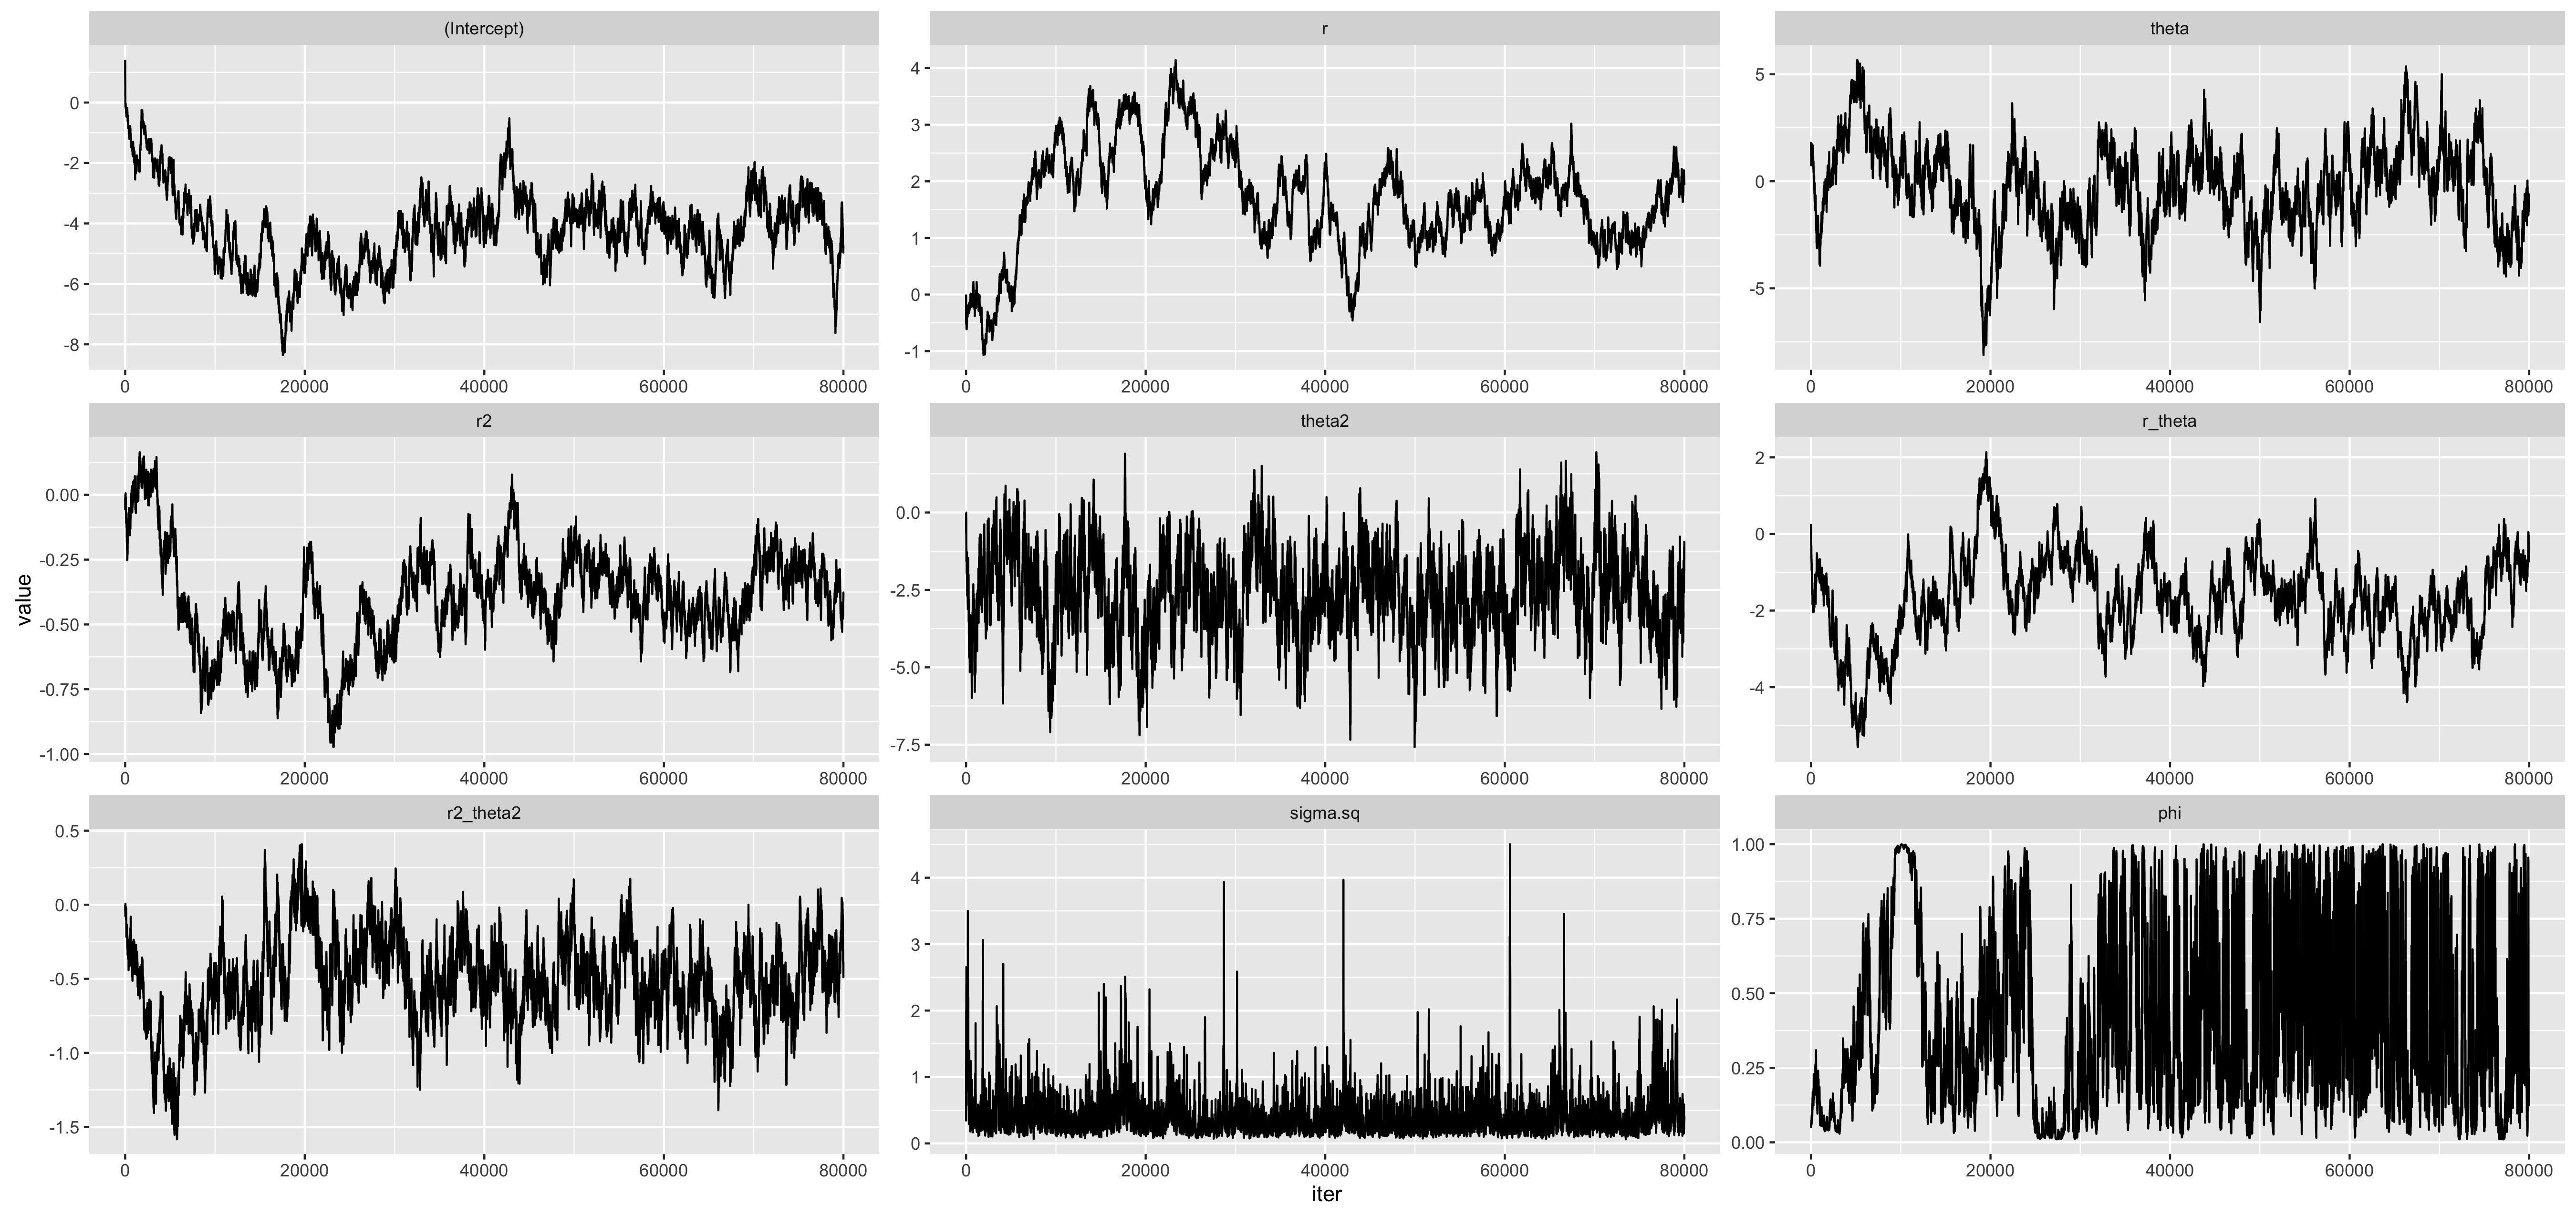
\includegraphics[scale=.1]{n3000.jpeg} 
\begin{itemize}
      

\item Need to think. Digest. Good progress.
\item Recall: Stan guys suggested identifiability and convergence issues can result from... something. Should look back at what they said. 
\item Stan implementation online uses version from ``Improved...'' follow-up paper Finley wrote.
\end{itemize}

\subsection*{Shiny it Up!}
\begin{itemize}
\item Two heat maps to Shiny: 
  \begin{enumerate}
  \item Empirical Var Res; Normal approx. to Binomial: $\hat{p} \pm z_{1-\alpha/2}*\sqrt{\hat{p}(1-\hat{p})/n}$
  \item Polar model (w/o random effect); each point has its own SE; MLE estimates are Normally distributed (gotta double check in GLM text); use \verb|predict()| function; use \verb|Field_of_Dreams3.R| as a reference; SE of the fit is calculated, so only new $z_{1-\alpha/2}$ will need to be plugged into fit $\pm z_{1-\alpha/2}*$se.fit each time
  \end{enumerate}
\item Not gonna be too bad.
\item Confusing the heck out of me. Review.
  \begin{itemize}
  \item $\alpha$ = P(No coverage)
  \item CI\% = 1 - $\alpha$
  \item $P(Z > z_{\alpha}) = \alpha$ 
  \begin{verbatim}
  > qnorm(0.05, lower.tail = FALSE)
  [1] 1.644854
  \end{verbatim}
  So $P(Z > 1.645) = 0.05$. Think of Normal curve. 
  \item For 95\% CI, we say $\alpha = 0.05$.
        \begin{itemize}
        \item This necessitates $z_{1-\alpha/2}$ for CI.
        \item $\hat{p} \pm z_{1-\alpha/2}*\sqrt{\hat{p}(1-\hat{p})/n}$
        \end{itemize}


  \end{itemize}
\item I got... my Shiny app... TO WORK!!! 
\end{itemize}

\subsection*{Meeting}

\subsubsection*{Items to report}
\begin{itemize}
\item Mango interview, R Coding Test
  \begin{itemize}
  \item Alix: progress updates! Tell them if anything happens. 
  \item Definitely give them a heads up if they are going to get a call (as a reference).
  \item Alix said: ``You're one of the most curious people I've ever met. It's a great part of who you are. Always reading all those books, walking around with... [imitates fiddlink] in your hand.'' She said I could/should have added that to my well-rounded answer.
  \item Charlotte/Alix said the same job here (statistical consultant) would bring in \$120,000 - \$140,000
  \end{itemize}
\item Heat Map CI Shiny app
  \begin{itemize}
  \item Add simple, point and click CI??? (Charlotte's challenge)
  \end{itemize}
\item spBayes works-ish, trace plots
  \begin{itemize}
  \item Trace plots indicate non-convergence, but this should not discourage, but instead encourage more iterations. More more more iterations. 
  \item Also keep in mind we're reducing information in some way, using knots only.
  \item Both thought 97 was a lot.
  \item Alix very excited it's working. ``Andy is going to be so excited; we're using his package on baseball data!''
  \end{itemize}
\end{itemize}

\subsection*{Evaluate Inverse you say?? Yes.}
\begin{itemize}
\item logit\{EY(s)\} = $\pmb{X}(s)\pmb{\beta} + Z(s)$, with $Z(s) \sim MVN\{\pmb{0}, \Sigma_{s}\}$
\item $f(\pmb{\beta}, \phi, \sigma^{2}, \pmb{Z}|\pmb{Y}) \propto f(\pmb{Y}|\pmb{\beta}, \phi, \sigma^{2}, \pmb{Z})f(\pmb{\beta})f(\pmb{Z}|\phi, \sigma^{2})f(\phi)f(\sigma^{2})$
\item M-H proposal, iteration i: $Z_{10,i}$
$$ r = \frac{ f(Z_{10,i}|\pmb{Z}_{1:9,i},\pmb{Z}_{11:n,i-1}, \pmb{\beta}_{i-1}, \phi_{i}, \sigma^{2}_{i})}{f(Z_{10,i-1}|\pmb{Z}_{1:9,i},\pmb{Z}_{11:n,i-1}, \pmb{\beta}_{i-1}, \phi_{i}, \sigma^{2}_{i})} $$
 
\item Note: $f(z_{1}, z_{2}, z_{3}|\pmb{Y}) = f(z_{1}|z_{2},z_{3},\pmb{Y})f(z_{2},z_{3}|\pmb{Y})$. So... $$r \propto \frac{f(\pmb{Y}|\pmb{\theta}_{i})f(\pmb{\beta})f(Z_{10,i}|\pmb{Z}_{1:9,i},\pmb{Z}_{11:n,i-1}, \phi_{i}, \sigma^{2}_{i})f(\pmb{Z}_{1:9,i},\pmb{Z}_{11:n,i-1}|\phi_{i}, \sigma^{2}_{i})f(\phi)f(\sigma^{2})} {f(\pmb{Y}|\pmb{\theta}_{i-1})f(\pmb{\beta})f(Z_{10,i-1}|\pmb{Z}_{1:9,i},\pmb{Z}_{11:n,i-1}, \phi_{i}, \sigma^{2}_{i})f(\pmb{Z}_{1:9,i},\pmb{Z}_{11:n,i-1}|\phi_{i}, \sigma^{2}_{i})f(\phi)f(\sigma^{2})}$$

$$ r \propto \frac{f(\pmb{Y}|\pmb{\theta}_{i})f(Z_{10,i}|\pmb{Z}_{1:9,i},\pmb{Z}_{11:n,i-1}, \phi_{i}, \sigma^{2}_{i})}
{f(\pmb{Y}|\pmb{\theta}_{i-1})f(Z_{10,i-1}|\pmb{Z}_{1:9,i},\pmb{Z}_{11:n,i-1}, \phi_{i}, \sigma^{2}_{i})} $$

\item And $f(\pmb{Z})$, $f(Z_{i}|\pmb{Z}_{-i})$, etc. are $MVN\{\cdot,\Sigma^{*}\}$, where $\Sigma^{*}$ either is, or is some function of, $\Sigma_{\pmb{s}}$; with PDF kernal containing $\Sigma_{\pmb{s}}^{*-1}$, (containing $\phi_{i}, \sigma^{2}_{i})$.

\end{itemize}

\subsection*{Next Steps}
\begin{itemize}
\item Convergence, more iterations for \verb|m1 <- spGLM(...)|
\item Add Charlotte requested feature to Shiny app
\item Add var. res. map to shiny app
\item Write. Add ending to chapter one. Start chapter two: introduce random effect, SPGLMM, stan/dimensionality issues/refinement (appendix?), Finley predictive process model dimension reduction
\item Fit predictive process model in Stan?
\end{itemize}

\section*{February 6, 2017}

\begin{itemize}
\item Fit predictive process model in Stan. 
        \begin{itemize}
        \item \citep{Neal2011} Figure 5.4, Figure 5.5, Figure 5.6 illustrate the much better, {\it smarter} mixing with HMC over random-walk Metropolis.
        \item Samples more correlated from random-walk Metropolis \citep{Neal2011}
        \item Speed (LondonR rstan presentation)
        \item No-U-Turn sampler \citep{Hoffman2014}; 
        \item rstan: ``full Bayesian inference using the No-U-Turn sampler (NUTS), a variant of Hamiltonian Monte
Carlo (HMC)'' \citep{rSTANtheMan}
        \end{itemize}
\item Idea of day: Collapse all locations to knot locations, estimate $\phi$ and $\sigma^{2}$. What else?
\item Going to try to create $N \times M$ covariance(obs, knots) matrix in stan; pg 387 in Stan the Manual; did it. 
\item Random side-note - {\bf Clayton Copulas} look like my hit distribution.
\item Maybe we should do a WAY BETTER JOB of what Cross and Sylvan did. Use league averages, exponential covariance structure with predictive process model knots to estimate covariance parameters. Get rid of hokey r, $\theta$ business.
\item Could have Ben show me how to access the mysterious, high power processors we have access to.
\end{itemize}

\subsection*{Knot Selection} % =====================================
\citep{Banerjee2008}
\begin{itemize}
\item In forest biomass example \cite{Banerjee2008} says ``With only 36 knots the distance between adjacent knots (40 km) seemed to exceed the effective spatial ranges that were supported by the data and {\bf led to unreliable convergence of process parameters}.'' (Boldface mine)
\item ``...knot selection is required and as we demonstrated in Section 5.1 some sensitivity to the number of knots is expected. Although for most applications a reasonable grid of knots should lead to robust inference, with {\bf fewer knots} the separation between them increases and estimating random fields with {\bf fine scale spatial} dependence becomes {\bf difficult}. Indeed, learning about {\bf fine scale spatial dependence} is always a {\bf challenge} (see, for example, Cressie (1993), page 114).'' (boldface mine)
\end{itemize}

\subsection*{Meeting}
Charlotte
\begin{itemize}
\item Get around ``for'' loop somehow?
\item Try binning distances idea?
\item Look at HMC convergence more closely, make sure this is worth it.
\item Websites for HTML/CSS (Codeacademy), \\ C++ (http://adv-r.had.co.nz/Rcpp.html), \\ GitHub (http://happygitwithr.com/)
\end{itemize}
Alix
\begin{itemize}
\item Email Debashis again if I feel like it, drop Alix's name
\item {\bf Anything in paper about how to choose the number of knots? Look into it.}
\item Just choose a hitter with fewer swings. Russian pencil method.
\item Try with way fewer knots. Ten knots.
\item Email Andy if I feel like it.
\item Alix doesn't want to try the aggregating thing yet, says I haven't struggled with predictive process models enough yet. (Admittedly, it has only been a few weeks or so)
\item Fix $\beta$s, estimate covariance parameters? Try it.
\item Start thinking about cross-validation.
\item Run the long, five hour estimations, do something else while it goes.
\item Alix thinks--and I reluctantly agree--that sometimes I am too quick to say "good enough." ...as I was with package question on the Mango ``R Coding Test.''
\end{itemize}

\subsection*{Fix Covariates}
\begin{itemize}
\item spBayes, n=3000, one chain, 37500 iteration
\begin{verbatim}
           Mean     SD  Naive SE Time-series SE
XB       1.0000 0.0000 0.0000000       0.000000
sigma.sq 0.2921 0.1850 0.0009551       0.006772
phi      0.4318 0.2886 0.0014905       0.032011
\end{verbatim}
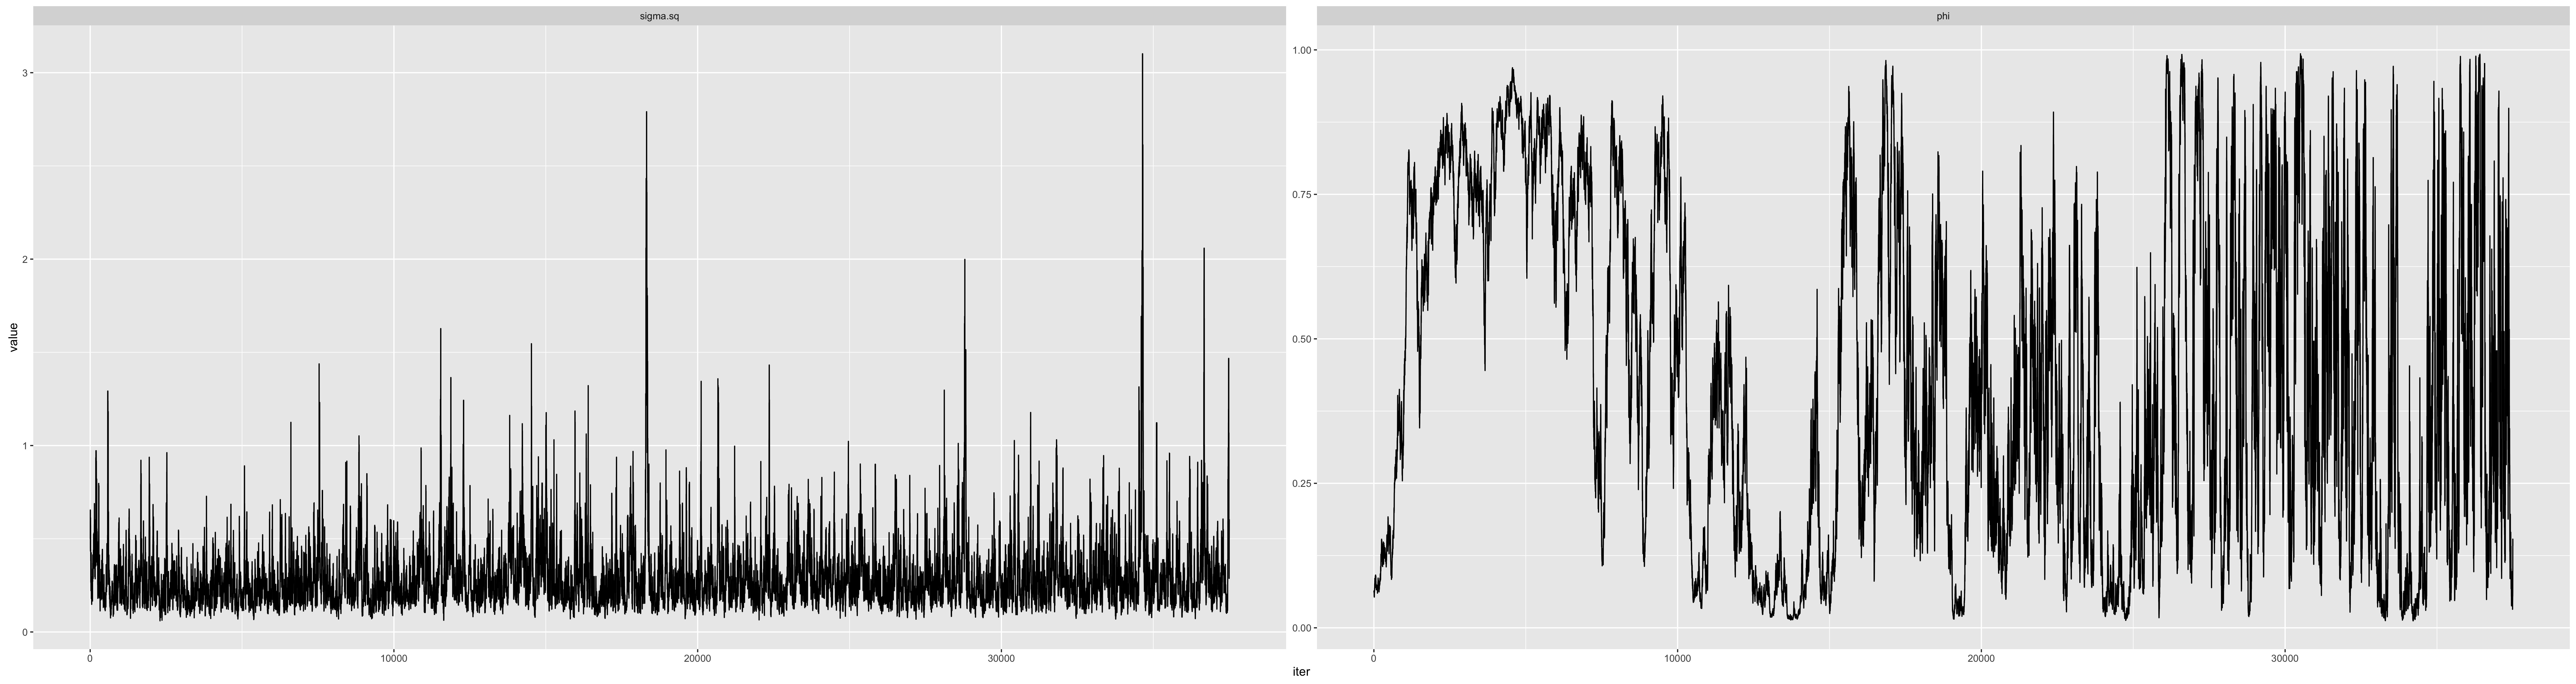
\includegraphics[scale=.05]{Images/n3000_XB.jpeg} \\

\end{itemize}

\section*{February 13, 2017}

\subsection*{Miscellaneous}
\begin{itemize}
\item Diagnose convergence
\item ``As with any knot based method, selection of knots is a challenging problem... Suppose for the moment that $m$ is given. We are essentially dealing with a problem that is analogous to a {\bf spatial design problem}...'' \citep{Finley2009}
\item {\bf Spatial design problem}
\item ``There is a rich literature in spatial design with is summarized in, e.g., the recent paper of \cite{Xia2006}''
\item ``Approximately optimal spatial design approaches for environmental health data.'' \citep{Xia2006}
\item ``Spatial sampling design for parameter estimation of the covariance function'' \citep{Zhu2005}
\end{itemize}

% ================= ================ ================= =============== =========
\subsection*{``Hierarchical Spatial Models... ''\citep{Finley2009_2}; multinomial}
\begin{itemize}
\item ``While most of the models we formulate can possibly be estimated using maximum likelihood or variants thereof, we adopt a Bayesian approach [e.g., Gelfand et al. (2003)]. This is attractive, as it offers exact inference for the random spatial coefficients, and that too with non-Gaussian data, by delivering an entire posterior distribution at both observed and unobserved locations. Spatial interpolation for processes that are neither observed nor arise as residuals appears inaccessible with classical likelihood-based methods. On the other hand, Bayesian model fitting involves rather specialized Markov chain Monte Carlo (MCMC) methods [see, e.g., Robert and Casella (2005)] that raise concerns about computational expense and reproducibility of inference. These concerns have, however, started to wane with the delivery of relatively simpler R packages (www.r-project.org), including mcmc, MCMCpack, geoRglm and spBayes, that help automate such methods and diagnose convergence.''
\item ``While our primary contribution here lies in the novel application, we also offer several methodological advancements.''
\item ``Three MCMC chains of 75,000 iterations were run for each model. Then posterior inference was based on 3 × 50,000 = 150,000 post burn-in samples.''
\item Justifications (pg 7) for PPMs over other methods, for dealing with large spatial datasets: (i) adapts easily to multivariate processes, (ii) spatial interpolation convenient, (iii) non-Gaussian, (iv) Flexible, multi-parameter with several hyperparameters (over INLA, Integrated Nested Laplace Approximations)
\item ``With irregular locations, however, we may encounter substantial areas of sparse observations where placing would amount to “wastage,” possibly leading to inflated variance estimates and slower convergence. More practical space-covering designs [e.g., Royle and Nychka (1998)] can yield a representative collection of knots that better cover the domain.''
    \begin{itemize}
    \item This could be a contribution. Compare my ``var-res-grid centers as knots'' to Nychka.
    \end{itemize}
\item ``We consider several different scoring rules to evaluate the predictive performance of the candidate models. A scoring rule provides a summary measure for evaluating a probabilistic prediction given the predictive distribution and the observed outcome. '' pg 10
\item ``\cite{Gneiting2007} offer four scoring rules for prediction of categorical variables'' page 10. 
  \begin{itemize}
  \item These guys have other papers, and LOTS of citations.
  \end{itemize}
\item {\bf Confusion matrix} - (google search) A confusion matrix is a table that is often used to describe the performance of a classification model (or "classifier") on a set of test data for which the true values are known. (google search)
\item ``We also compare our spatially-varying multinomial logistic regression models to common benchmark methods'' page 11
\item ``For estimating predicive process models, we used 154, 200, and 254 knots over the domain.''
  \begin{itemize}
  \item Could the efficacy of the PPM with X knots inform, in reverse, a method for choosing the cutoff?
  \end{itemize}
\item ``The spatially-varying coefficients model was the most computationally challenging, with each chain of the 254 knot model taking ~5 hours to complete. {\bf The \verb|CODA| package in R (www.r-project.org) was used to diagnose convergence by monitoring mixing using Gelman–Rubin diagnostics and autocorrelations} [see, e.g., Gelman et al. (2004), Section 11.6]. Acceptable convergence was diagnosed within 25,000 iterations and, therefore, 150,000 samples (3 x 50,000) were retained for posterior analysis.''
  \begin{itemize}
  \item DIAGNOSTICS. 
  \end{itemize}
\end{itemize}

\subsection*{Meeting}
\begin{itemize}
\item I think ``var-res-grid centers as knots'' is viable. I could compare to \cite{Nychka1998}. Could/should this be a (Ch 2? Ch 3) contribution? 
\end{itemize}

\subsection*{Where are we? What's our depth?!} % ============= ============ ========
\begin{itemize}
\item Var-Res heat maps
  \begin{itemize}
  \item Heat maps
  \item Shiny
  \end{itemize}
\item MLE model
  \begin{itemize}
  \item Profile plots to show interpretability potential
  \end{itemize}
\item Random effect model
  \begin{itemize}
  \item MCMC - Markov Chain Monte Carlo
  \item Stan - HMC
          \begin{itemize}
          \item Code code code (communications, and Trangucci2017 handout)
          \item Hamiltonian Monte Carlo \citep{Neal2011}
          \end{itemize}
  \item spBayes, Predictive process models
          \begin{itemize}
          \item Knot quantity - seems like comparison at range of values
          \item placement decisions - my var-res-grid centers vs. \citep{Nychka1998}
          \item Metropolis nuts and bolts
          \item {\bf Convergence} - \cite{Finley2011} talks about convergence, Gelman-Rubin diagnostics (\citep{Gelman2014}), mixing, and \verb|CODA| package in R, classification confusion matrix, on page 12.
          \end{itemize}
  \end{itemize}
\item Include Cross kriging, empirical Bayes boxes
\item Model validation, comparison
      \begin{itemize}
      \item Hosmer-Lemeshow - goodness of fit test
      \item \cite{Finley2011} has ``5.1 Model validation and benchmark comparisons'' section
      \item \cite{Finley2011} cites \cite{Gneiting2007} regarding scoring rules, etc., as have 1577 other papers
      \end{itemize}
\end{itemize}

% \bibliographystyle{plainnat}
\bibliography{Baseball}



\end{document}